\documentclass[aspectratio=43]{beamer}

% Text packages to stop warnings
\usepackage{lmodern}
\usepackage{tikz}
\usepackage{textcomp}
\usepackage[utf8]{inputenc}
\usepackage[T1]{fontenc}
\usepackage{ulem}
\usepackage{listings}

\usetikzlibrary{arrows,automata,shapes}
\tikzstyle{block} = [rectangle, draw, fill=blue!20, 
    text width=2.5em, text centered, rounded corners, minimum height=2em]
\tikzstyle{bw} = [rectangle, draw, fill=blue!20, 
    text width=3.5em, text centered, rounded corners, minimum height=2em]

% Themes
\usetheme{Boadilla}
\setbeamertemplate{footline}[page number]{}
\setbeamertemplate{navigation symbols}{}

% Suppress the navigation bar
\beamertemplatenavigationsymbolsempty

\newenvironment{changemargin}[1]{% 
  \begin{list}{}{% 
    \setlength{\topsep}{0pt}% 
    \setlength{\leftmargin}{#1}% 
    \setlength{\rightmargin}{1em}
    \setlength{\listparindent}{\parindent}% 
    \setlength{\itemindent}{\parindent}% 
    \setlength{\parsep}{\parskip}% 
  }% 
  \item[]}{\end{list}} 

\lstset{basicstyle=\scriptsize, frame=single}

\title{Lecture 36---Massive Scalability; Course Summary}
\subtitle{ECE 459: Programming for Performance}
\date{April 6, 2015}

\begin{document}
%%%%%%%%%%%%%%%%%%%%%%%%%%%%%%%%%%%%%%%%%%%%%%%%%%%%%%%%%%%%%%%%%%%%%%%%%%%%%%%%
\begin{frame}[plain]
  \titlepage
\end{frame}
%%%%%%%%%%%%%%%%%%%%%%%%%%%%%%%%%%%%%%%%%%%%%%%%%%%%%%%%%%%%%%%%%%%%%%%%%%%%%%%%

%%%%%%%%%%%%%%%%%%%%%%%%%%%%%%%%%%%%%%%%%%%%%%%%%%%%%%%%%%%%%%%%%%%%%%%%%%%%%%%%
\part{Clusters vs Laptops}
\frame{\partpage}
%%%%%%%%%%%%%%%%%%%%%%%%%%%%%%%%%%%%%%%%%%%%%%%%%%%%%%%%%%%%%%%%%%%%%%%%%%%%%%%%

%%%%%%%%%%%%%%%%%%%%%%%%%%%%%%%%%%%%%%%%%%%%%%%%%%%%%%%%%%%%%%%%%%%%%%%%%%%%%%%%
\begin{frame}
  \frametitle{References}

  \begin{changemargin}{1cm}
{\Large
Frank McSherry, Michael Isard, Derek G. Murray. ``Scalability! But at what COST?'' \\
To appear in Proceedings of HotOS XV.\\[1em]}

The blog post is more digestible:\\
  \end{changemargin}
{\scriptsize
\hspace*{1cm} \url{http://www.frankmcsherry.org/graph/scalability/cost/2015/01/15/COST.html}
}
\end{frame}
%%%%%%%%%%%%%%%%%%%%%%%%%%%%%%%%%%%%%%%%%%%%%%%%%%%%%%%%%%%%%%%%%%%%%%%%%%%%%%%%

%%%%%%%%%%%%%%%%%%%%%%%%%%%%%%%%%%%%%%%%%%%%%%%%%%%%%%%%%%%%%%%%%%%%%%%%%%%%%%%%
\begin{frame}
  \frametitle{Problem: Overhead}
  \begin{changemargin}{2cm}
\Large
    Scaling to ``big data'' systems\\
    introduces substantial overhead.\\[1em]

    How much?\\
 Let's do a head-to-head comparison!
  \end{changemargin}
\end{frame}
%%%%%%%%%%%%%%%%%%%%%%%%%%%%%%%%%%%%%%%%%%%%%%%%%%%%%%%%%%%%%%%%%%%%%%%%%%%%%%%%

%%%%%%%%%%%%%%%%%%%%%%%%%%%%%%%%%%%%%%%%%%%%%%%%%%%%%%%%%%%%%%%%%%%%%%%%%%%%%%%%
\begin{frame}[fragile]
  \frametitle{The Experiment}
{\tiny \begin{verbatim}citation: "Macbook Pro Retina 13 2013" by TechGizmo - Own work. 
Licensed under CC BY-SA 3.0 via Wikimedia Commons - 
http://commons.wikimedia.org/wiki/File:Macbook_Pro_Retina_13_2013.jpg
\end{verbatim}
}
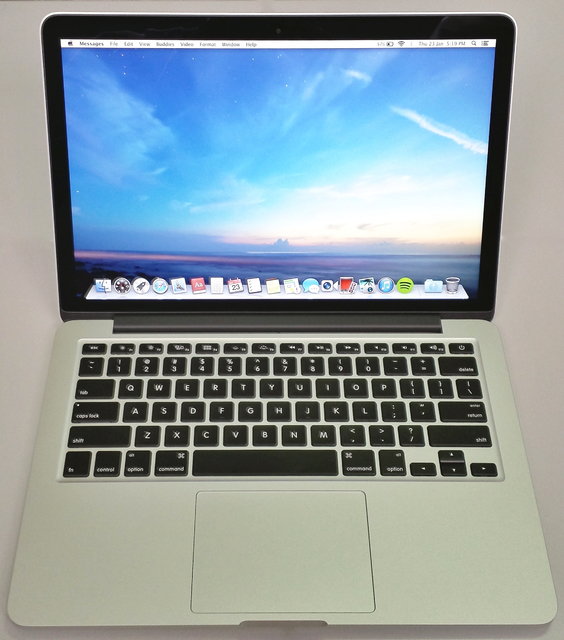
\includegraphics[height=.4\textheight]{L36/Macbook_Pro_Retina_13_2013.jpg}
 \hspace*{1cm} vs \hspace*{1cm}
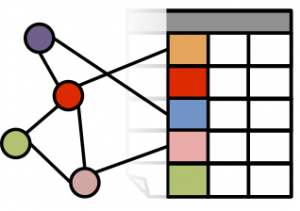
\includegraphics[height=.3\textheight]{L36/table_and_graph-300x211.png}
(GraphX)
\end{frame}
%%%%%%%%%%%%%%%%%%%%%%%%%%%%%%%%%%%%%%%%%%%%%%%%%%%%%%%%%%%%%%%%%%%%%%%%%%%%%%%%


%%%%%%%%%%%%%%%%%%%%%%%%%%%%%%%%%%%%%%%%%%%%%%%%%%%%%%%%%%%%%%%%%%%%%%%%%%%%%%%%
\begin{frame}
  \frametitle{Conclusion}

\begin{quote}
Big data systems haven't yet been shown to be obviously good; current evaluation is lacking.
\end{quote}

  \begin{changemargin}{0.5cm}
\begin{tabbing}
Takeaway: \= The important metric is not just scalability;\\
\> absolute performance matters a lot too.
\end{tabbing}
  \end{changemargin}
\end{frame}
%%%%%%%%%%%%%%%%%%%%%%%%%%%%%%%%%%%%%%%%%%%%%%%%%%%%%%%%%%%%%%%%%%%%%%%%%%%%%%%%


%%%%%%%%%%%%%%%%%%%%%%%%%%%%%%%%%%%%%%%%%%%%%%%%%%%%%%%%%%%%%%%%%%%%%%%%%%%%%%%%
\begin{frame}
  \frametitle{Methodology}
  \begin{changemargin}{2cm}

Laptop vs. Big Data systems (GraphX).

Domain: Graph Processing algorithms.\\
\begin{itemize}
\item PageRank (sparse matrix/vector multiplication)
\item graph connectivity (label propagation)
\end{itemize}

Subject: graphs with billions of edges (few GBs of data).

  \end{changemargin}
\end{frame}
%%%%%%%%%%%%%%%%%%%%%%%%%%%%%%%%%%%%%%%%%%%%%%%%%%%%%%%%%%%%%%%%%%%%%%%%%%%%%%%%

%%%%%%%%%%%%%%%%%%%%%%%%%%%%%%%%%%%%%%%%%%%%%%%%%%%%%%%%%%%%%%%%%%%%%%%%%%%%%%%%
\begin{frame}
  \frametitle{Results}
  \begin{changemargin}{1cm}
Twenty pagerank iterations:
\hspace*{.5cm}\begin{tabular}{lrrr}
System &cores 	&twitter\_rv 	&uk\_2007\_05\\ \hline
Spark 	&128 	&857s 	&1759s\\
Giraph 	&128 	&596s 	&1235s\\
GraphLab 	&128 	&249s 	&833s\\
GraphX 	&128 	&419s 	&462s\\
Single thread 	&1 	&300s	&651s
\end{tabular}
~\\[1em]
Label propagation to fixed-point (graph connectivity)
\hspace*{.5cm}\begin{tabular}{lrrr}
System 	&cores 	&twitter\_rv 	&uk\_2007\_05\\ \hline
Spark 	&128 	&1784s 	&8000s+\\
Giraph 	&128 	&200s 	&8000s+\\
GraphLab 	&128 	&242s 	&714s\\
GraphX 	&128 	&251s 	&800s\\
Single thread 	&1 	&153s	&417s
\end{tabular}

%\item 128 cores don't consistently beat a laptop at PageRank;\\
%249--857s on the twitter\_rv dataset for the big data system vs 300s for the laptop.\\
%2$\times$ slower for label propagation, at 251--1784s for the big data system vs 153s on
%twitter\_rv.

%(See the blog post for the full results).
  \end{changemargin}
\end{frame}
%%%%%%%%%%%%%%%%%%%%%%%%%%%%%%%%%%%%%%%%%%%%%%%%%%%%%%%%%%%%%%%%%%%%%%%%%%%%%%%%

%%%%%%%%%%%%%%%%%%%%%%%%%%%%%%%%%%%%%%%%%%%%%%%%%%%%%%%%%%%%%%%%%%%%%%%%%%%%%%%%
\begin{frame}
  \frametitle{Algorithmic Improvements}
  \begin{changemargin}{1cm}
Algorithmic improvements can win big.\\
(Hard to generalize, though.)\\[1em]

Examples:
\begin{itemize}
\item Hilbert curves for data layout improve memory locality\\
(helps a lot for PageRank); and
\item  using a union-find algorithm (also parallelizable).\\
 ``10$\times$ faster, 100$\times$ less embarrassing''. 
\end{itemize}

\begin{tabbing}
Results: overall, \= $2\times$ speedup for PageRank and\\
\> $10\times$ speedup for label propagation.
\end{tabbing}

  \end{changemargin}
\end{frame}
%%%%%%%%%%%%%%%%%%%%%%%%%%%%%%%%%%%%%%%%%%%%%%%%%%%%%%%%%%%%%%%%%%%%%%%%%%%%%%%%

%%%%%%%%%%%%%%%%%%%%%%%%%%%%%%%%%%%%%%%%%%%%%%%%%%%%%%%%%%%%%%%%%%%%%%%%%%%%%%%%
\begin{frame}
  \frametitle{Takeaways}
  \begin{changemargin}{1cm}

\begin{itemize}
\item    ``If you are going to use a big data system for yourself, \\ see if it is faster than your laptop.''
\item    ``If you are going to build a big data system for others, \\ see that it is faster than my laptop.''
\end{itemize}

  \end{changemargin}
\end{frame}
%%%%%%%%%%%%%%%%%%%%%%%%%%%%%%%%%%%%%%%%%%%%%%%%%%%%%%%%%%%%%%%%%%%%%%%%%%%%%%%%

%%%%%%%%%%%%%%%%%%%%%%%%%%%%%%%%%%%%%%%%%%%%%%%%%%%%%%%%%%%%%%%%%%%%%%%%%%%%%%%%
\part{Massive Scalability}
\frame{\partpage}
%%%%%%%%%%%%%%%%%%%%%%%%%%%%%%%%%%%%%%%%%%%%%%%%%%%%%%%%%%%%%%%%%%%%%%%%%%%%%%%%

%%%%%%%%%%%%%%%%%%%%%%%%%%%%%%%%%%%%%%%%%%%%%%%%%%%%%%%%%%%%%%%%%%%%%%%%%%%%%%%%
\begin{frame}
  \frametitle{People worth following}

  \begin{changemargin}{2cm}
\Large
  \begin{itemize}
    \item Fran Allen (IBM)
    \item Jeff Dean (Google)
    \item Keith Packard (Intel)
    \item Herb Sutter (Microsoft)
  \end{itemize}
  \end{changemargin}
\end{frame}
%%%%%%%%%%%%%%%%%%%%%%%%%%%%%%%%%%%%%%%%%%%%%%%%%%%%%%%%%%%%%%%%%%%%%%%%%%%%%%%%

%%%%%%%%%%%%%%%%%%%%%%%%%%%%%%%%%%%%%%%%%%%%%%%%%%%%%%%%%%%%%%%%%%%%%%%%%%%%%%%%
\begin{frame}
  \frametitle{Some Thoughts from Jeff Dean}

  \begin{changemargin}{2cm}
    URL: \url{research.google.com/pubs/jeff.html}\\[1em]

    Selections from:\\
    ``Software Engineering Advice for Building\\
\qquad  Large-Scale Distributed Systems''.\\[1em]

    On scaling:
\begin{itemize}
  \item design for $\sim$ 10x, rewrite before 100x
\end{itemize}
~\\

    Key concept for scaling:
\begin{itemize}
  \item sharding, also known as partitioning.
\end{itemize}

  \end{changemargin}
\end{frame}
%%%%%%%%%%%%%%%%%%%%%%%%%%%%%%%%%%%%%%%%%%%%%%%%%%%%%%%%%%%%%%%%%%%%%%%%%%%%%%%%

%%%%%%%%%%%%%%%%%%%%%%%%%%%%%%%%%%%%%%%%%%%%%%%%%%%%%%%%%%%%%%%%%%%%%%%%%%%%%%%%
\begin{frame}
  \frametitle{Why Distribute?}

  \begin{changemargin}{2cm}
    Let's say that we want a copy of the Web.\\[1em]

    20+ billion web pages $\times$ 20KB = 400+ TB.\\
    $\qquad \sim$ 3 months to read the web.\\
    $\qquad \sim$ 1000 HDs (in 2010) to store the web.\\[1em]

    And that's without even processing the data!

  \end{changemargin}
\end{frame}
%%%%%%%%%%%%%%%%%%%%%%%%%%%%%%%%%%%%%%%%%%%%%%%%%%%%%%%%%%%%%%%%%%%%%%%%%%%%%%%%

%%%%%%%%%%%%%%%%%%%%%%%%%%%%%%%%%%%%%%%%%%%%%%%%%%%%%%%%%%%%%%%%%%%%%%%%%%%%%%%%
\begin{frame}
  \frametitle{Magic solution: distribute the problem!}

  \begin{changemargin}{2cm}
    1000 machines $\Rightarrow ~< 3$ hours.\\[1em]

    No Free Lunch.\\
    Problems: need to deal with \ldots \\
\begin{itemize}
  \item communication \& coordination;
  \item recovering from machine failure;
  \item status reporting;
  \item debugging;
  \item optimization;
  \item locality
\end{itemize}

   \ldots and that, from scratch, for each problem!
  \end{changemargin}
\end{frame}
%%%%%%%%%%%%%%%%%%%%%%%%%%%%%%%%%%%%%%%%%%%%%%%%%%%%%%%%%%%%%%%%%%%%%%%%%%%%%%%%

%%%%%%%%%%%%%%%%%%%%%%%%%%%%%%%%%%%%%%%%%%%%%%%%%%%%%%%%%%%%%%%%%%%%%%%%%%%%%%%%
\begin{frame}
  \frametitle{Designing Systems as Services/Platforms}

\qquad \qquad Steve Yegge on Google and Platforms:
\begin{center}
\scriptsize \url{https://plus.google.com/112678702228711889851/posts/eVeouesvaVX}
\end{center}

  \begin{changemargin}{1cm}
\small
[Bezos's] Big Mandate went something along these lines:

1) All teams will henceforth expose their data and functionality through service interfaces.

2) Teams must communicate with each other through these interfaces.

3) There will be no other form of interprocess communication allowed: no direct linking, no direct reads of another team's data store, no shared-memory model, no back-doors whatsoever. The only communication allowed is via service interface calls over the network.

4) It doesn't matter what technology they use. HTTP, Corba, Pubsub, custom protocols -- doesn't matter. Bezos doesn't care.

5) All service interfaces, without exception, must be designed from the ground up to be externalizable. That is to say, the team must plan and design to be able to expose the interface to developers in the outside world. No exceptions.

6) Anyone who doesn't do this will be fired.

7) Thank you; have a nice day! [j/k]
  \end{changemargin}
\end{frame}
%%%%%%%%%%%%%%%%%%%%%%%%%%%%%%%%%%%%%%%%%%%%%%%%%%%%%%%%%%%%%%%%%%%%%%%%%%%%%%%%

%%%%%%%%%%%%%%%%%%%%%%%%%%%%%%%%%%%%%%%%%%%%%%%%%%%%%%%%%%%%%%%%%%%%%%%%%%%%%%%%
\begin{frame}
  \frametitle{Why Services?}
  \begin{changemargin}{2cm}
    Decouple different parts of a system.\\[1em]

    ``Fewer dependencies, clearly specified''.\\[1em]

    ``Easy to test new versions.''\\[1em]

    ``Small teams can work independently.''
  \end{changemargin}
\end{frame}
%%%%%%%%%%%%%%%%%%%%%%%%%%%%%%%%%%%%%%%%%%%%%%%%%%%%%%%%%%%%%%%%%%%%%%%%%%%%%%%%

%%%%%%%%%%%%%%%%%%%%%%%%%%%%%%%%%%%%%%%%%%%%%%%%%%%%%%%%%%%%%%%%%%%%%%%%%%%%%%%%
\begin{frame}
  \frametitle{How to Design Stuff}

  \begin{changemargin}{2cm}

    Talk to people!\\[1em]

    Write down a [some] rough sketch[es], \\ \qquad chat at a whiteboard.\\[1em]

    Design good interfaces. (This is hard.)

  \end{changemargin}
\end{frame}
%%%%%%%%%%%%%%%%%%%%%%%%%%%%%%%%%%%%%%%%%%%%%%%%%%%%%%%%%%%%%%%%%%%%%%%%%%%%%%%%

%%%%%%%%%%%%%%%%%%%%%%%%%%%%%%%%%%%%%%%%%%%%%%%%%%%%%%%%%%%%%%%%%%%%%%%%%%%%%%%%
\begin{frame}
  \frametitle{Using Back-of-the-Envelope Calculations I}

  \begin{changemargin}{2cm}
    ``How long to generate image results page (30 thumbnails)?''

    \begin{enumerate}
      \item read serially, thumbnail 256K images on-the-fly:\\
        30 seeks $\times$ 10 ms/seek + 30 $\times$ 256K / 30MB/s = 560ms

      \item issue reads in parallel:\\
        10 ms/seek + 256KB read / 30 MB/s = 18ms\\
        (plus variance: 30-60ms)
    \end{enumerate}
  \end{changemargin}
\end{frame}
%%%%%%%%%%%%%%%%%%%%%%%%%%%%%%%%%%%%%%%%%%%%%%%%%%%%%%%%%%%%%%%%%%%%%%%%%%%%%%%%

%%%%%%%%%%%%%%%%%%%%%%%%%%%%%%%%%%%%%%%%%%%%%%%%%%%%%%%%%%%%%%%%%%%%%%%%%%%%%%%%
\begin{frame}
  \frametitle{Using Back-of-the-Envelope Calculations II}

  \begin{changemargin}{1cm}
    ``How long to quicksort 1GB of 2-byte numbers?''\\[1em]

    Comparisons: lots of branch mispredicts.\\
    \quad log($2^{28}$) passes over $2^{28}$ numbers = $\sim 2^{33}$ compares\\
    \quad $\sim 50\%$ mispredicts = $2^{32}$ mispredicts $\times$ 5 ns/mispredict = 21s.\\[1em]

    Memory bandwidth: mostly sequential streaming.\\
    \quad $2^{30}$ bytes $\times ~28$ passes = 28GB; \\
    \quad memory bandwidth $\sim 4GB/s$, so $\sim 7$ seconds.\\[1em]

    Total: about 30 seconds to sort 1GB on 1 CPU.\\[1em]

    Also, write microbenchmarks. Understand your building blocks.

  \end{changemargin}
\end{frame}
%%%%%%%%%%%%%%%%%%%%%%%%%%%%%%%%%%%%%%%%%%%%%%%%%%%%%%%%%%%%%%%%%%%%%%%%%%%%%%%%


%%%%%%%%%%%%%%%%%%%%%%%%%%%%%%%%%%%%%%%%%%%%%%%%%%%%%%%%%%%%%%%%%%%%%%%%%%%%%%%%
\begin{frame}
  \frametitle{Numbers Everyone Should Know}

\begin{center}
\scriptsize \url{http://www.eecs.berkeley.edu/~rcs/research/interactive_latency.html}
\end{center}
\end{frame}
%%%%%%%%%%%%%%%%%%%%%%%%%%%%%%%%%%%%%%%%%%%%%%%%%%%%%%%%%%%%%%%%%%%%%%%%%%%%%%%%

\part{Course Summary}
\frame{\partpage}


%%%%%%%%%%%%%%%%%%%%%%%%%%%%%%%%%%%%%%%%%%%%%%%%%%%%%%%%%%%%%%%%%%%%%%%%%%%%%%%%
\begin{frame}
  \frametitle{Key Concepts I: goals}

  \begin{changemargin}{2cm}
  \begin{itemize}
  \item Bandwidth versus Latency.

  \item Concurrency versus Parallelism.

  \item More bandwidth through parallelism.

  \item Amdahl's Law and Gustafson's Law.
  \end{itemize}
  \end{changemargin}
\end{frame}
%%%%%%%%%%%%%%%%%%%%%%%%%%%%%%%%%%%%%%%%%%%%%%%%%%%%%%%%%%%%%%%%%%%%%%%%%%%%%%%%

%%%%%%%%%%%%%%%%%%%%%%%%%%%%%%%%%%%%%%%%%%%%%%%%%%%%%%%%%%%%%%%%%%%%%%%%%%%%%%%%
\begin{frame}
  \frametitle{Key Concepts II: leveraging parallelism}

  \begin{changemargin}{2cm}
  \begin{itemize}
    \item Features of modern hardware.

    \item Parallelism implementations: pthreads.
      \begin{itemize}
        \item definition of a thread;
        \item spawning threads.
      \end{itemize}

    \item Problems with parallelism: race conditions.
      \begin{itemize}
        \item manual solutions: mutexes, spinlocks, RW locks, semaphores, barriers.
        \item lock granuarlity.
      \end{itemize}

    \item Parallelization patterns; also SIMD.
  \end{itemize}
  \end{changemargin}
\end{frame}
%%%%%%%%%%%%%%%%%%%%%%%%%%%%%%%%%%%%%%%%%%%%%%%%%%%%%%%%%%%%%%%%%%%%%%%%%%%%%%%%

%%%%%%%%%%%%%%%%%%%%%%%%%%%%%%%%%%%%%%%%%%%%%%%%%%%%%%%%%%%%%%%%%%%%%%%%%%%%%%%%
\begin{frame}
  \frametitle{Key Concepts III: inherently-sequential problems}

  \begin{changemargin}{2cm}
  \begin{itemize}
    \item Barriers to parallelization: dependencies.
      \begin{itemize}
        \item loop-carried, memory-carried;
        \item RAW/WAR/WAW/RAR.
      \end{itemize}

    \item Breaking dependencies with speculation.
  \end{itemize}
  \end{changemargin}
\end{frame}
%%%%%%%%%%%%%%%%%%%%%%%%%%%%%%%%%%%%%%%%%%%%%%%%%%%%%%%%%%%%%%%%%%%%%%%%%%%%%%%%


%%%%%%%%%%%%%%%%%%%%%%%%%%%%%%%%%%%%%%%%%%%%%%%%%%%%%%%%%%%%%%%%%%%%%%%%%%%%%%%%
\begin{frame}
  \frametitle{Key Concepts IV: higher-level parallelization}

  \begin{changemargin}{2cm}
  \begin{itemize}
    \item Automatic parallelization; when does it work?

    \item Language/library support through OpenMP.
  \end{itemize}
  \end{changemargin}
\end{frame}
%%%%%%%%%%%%%%%%%%%%%%%%%%%%%%%%%%%%%%%%%%%%%%%%%%%%%%%%%%%%%%%%%%%%%%%%%%%%%%%%

%%%%%%%%%%%%%%%%%%%%%%%%%%%%%%%%%%%%%%%%%%%%%%%%%%%%%%%%%%%%%%%%%%%%%%%%%%%%%%%%
\begin{frame}
  \frametitle{Key Concepts V: hardware considerations}

  \begin{changemargin}{2cm}
  \begin{itemize}
    \item Unwelcome surprises: memory models \& reordering.
      \begin{itemize}
        \item fences and barriers; atomic instructions.
        \item cache coherency implementations.
      \end{itemize}
  \end{itemize}
  \end{changemargin}
\end{frame}
%%%%%%%%%%%%%%%%%%%%%%%%%%%%%%%%%%%%%%%%%%%%%%%%%%%%%%%%%%%%%%%%%%%%%%%%%%%%%%%%

%%%%%%%%%%%%%%%%%%%%%%%%%%%%%%%%%%%%%%%%%%%%%%%%%%%%%%%%%%%%%%%%%%%%%%%%%%%%%%%%
\begin{frame}
  \frametitle{Key Concepts VI: help from the compiler}

  \begin{changemargin}{2cm}
  \begin{itemize}
    \item Three-address code.
    \item Compiler constructs: volatile, restrict.
    \item Inlining and other static optimizations.
    \item Profile-guided optimizations.
  \end{itemize}
  \end{changemargin}
\end{frame}
%%%%%%%%%%%%%%%%%%%%%%%%%%%%%%%%%%%%%%%%%%%%%%%%%%%%%%%%%%%%%%%%%%%%%%%%%%%%%%%%

%%%%%%%%%%%%%%%%%%%%%%%%%%%%%%%%%%%%%%%%%%%%%%%%%%%%%%%%%%%%%%%%%%%%%%%%%%%%%%%%
\begin{frame}
  \frametitle{Key Concepts VII: profiling}

  \begin{changemargin}{2cm}
  \begin{itemize}
    \item Profiling tools and techniques.
    \item Call graphs, performance counters from profilers.
    \item When your profiler lies to you!
    \item Query-based DTrace approach.
  \end{itemize}
  \end{changemargin}
\end{frame}
%%%%%%%%%%%%%%%%%%%%%%%%%%%%%%%%%%%%%%%%%%%%%%%%%%%%%%%%%%%%%%%%%%%%%%%%%%%%%%%%

%%%%%%%%%%%%%%%%%%%%%%%%%%%%%%%%%%%%%%%%%%%%%%%%%%%%%%%%%%%%%%%%%%%%%%%%%%%%%%%%
\begin{frame}
  \frametitle{Key Concepts VIII: assorted topics}

  \begin{changemargin}{2cm}
  \begin{itemize}
    \item Reduced-resource computing.
    \item Software transactions.
    \item DevOps for programming for performance.
  \end{itemize}
  \end{changemargin}
\end{frame}
%%%%%%%%%%%%%%%%%%%%%%%%%%%%%%%%%%%%%%%%%%%%%%%%%%%%%%%%%%%%%%%%%%%%%%%%%%%%%%%%

%%%%%%%%%%%%%%%%%%%%%%%%%%%%%%%%%%%%%%%%%%%%%%%%%%%%%%%%%%%%%%%%%%%%%%%%%%%%%%%%
\begin{frame}
  \frametitle{Key Concepts IX: beyond single-core CPU programming}

  \begin{changemargin}{2cm}
  \begin{itemize}
    \item Languages for high-performance computing.
    \item GPU Programming (e.g. with OpenCL).
    \item Clusters: MapReduce, MPI.
    \item Clouds.
    \item Big Data.
  \end{itemize}
  \end{changemargin}
\end{frame}
%%%%%%%%%%%%%%%%%%%%%%%%%%%%%%%%%%%%%%%%%%%%%%%%%%%%%%%%%%%%%%%%%%%%%%%%%%%%%%%%

%%%%%%%%%%%%%%%%%%%%%%%%%%%%%%%%%%%%%%%%%%%%%%%%%%%%%%%%%%%%%%%%%%%%%%%%%%%%%%%%
\begin{frame}
  \frametitle{Final Words}

  \begin{changemargin}{2cm}
    Good luck on the final!
  \end{changemargin}
\end{frame}
%%%%%%%%%%%%%%%%%%%%%%%%%%%%%%%%%%%%%%%%%%%%%%%%%%%%%%%%%%%%%%%%%%%%%%%%%%%%%%%%

\end{document}
